\section{Ausgabe der Resultate}
\subsection{Erstellung des Ausgabeordners}
Alle ausgegebenen Dateien des Programms werden in einem Ordner zusammengefasst.
Dieser Ordner wird im gleichen Verzeichnis erstellt, in dem auch das Programm ausgeführt wird.
Als Name des Verzeichnisses wird der Name genutzt, den der Nutzer in der GUI eingegeben hat.
 
\begin{code}[Erstellung der Unterordner]
	private static void createDirs(String folderName) {
		try {
			Files.createDirectories(Paths.get("./" + folderName + "/scad"));
			Files.createDirectories(Paths.get("./" + folderName + "/stl"));
		} catch (IOException e) {
			e.printStackTrace();
		}
	}
\end{code}

Im Unterordner \q{scad} dieses Ordners finden sich dann sämtliche .scad-Dateien, im Unterordner \q{stl} alle .stl-Dateien.

\subsection{OpenSCAD Java Interface}
Für die erleichterte Erstellung von OpenScad Objekten wurde ein Java Interface \icode{ScadObject} erstellt, welches alle für das Projekt wichtigen Befehle enthält.
Die Methode \icode{toString()} stellt in den Klassen des Interfaces die Übergabe des OpenSCAD Befehlsstrings dar.
So kann man z.B. mit der Klasse \icode{Cube} einen Quader mit gegebener Länge, Höhe und Breite erstellen, der dann wie folgt mit \icode{Cube.toString()} in einen String konvertiert wird:
\icode{cube([Länge, Breite, Höhe]);}\\

\begin{Bild}{Resultat der Eingabe: \icode{new Cube(3, 4, 5).toString()} (Screenshot der Verfasser)}
	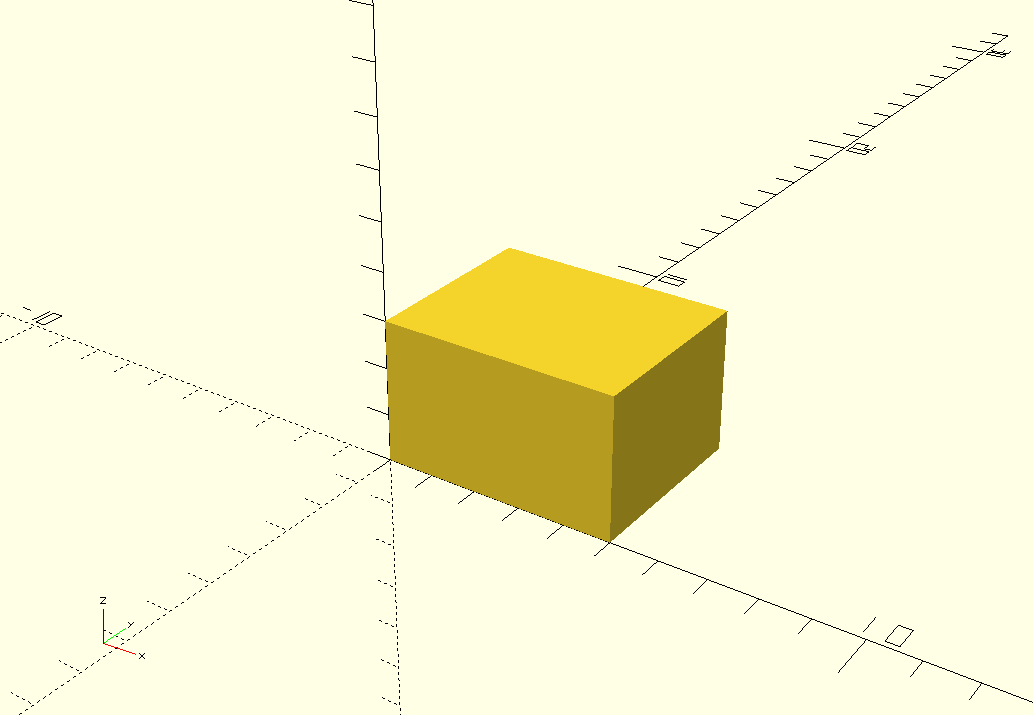
\includegraphics[height = 200px]{Bilder/Quader}
\end{Bild}

\subsection{STL Konvertierung}
Um die ermittelten .scad-Dateien im .stl-Format auszugeben, wird die Kommandozeilenfunktionalität von OpenSCAD verwendet.
Die verwendete Anweisung setzt sich hierbei aus dem Pfad zur \icode{openscad.exe}, dem Parameter \icode{-o} und zwei weiteren Parametern zusammen. 
Die beiden weiteren Parameter stehen zum einen für den Namen der Ausgabedatei und zum anderen für den Namen der Eingabedatei.
Eine vollständige Anweisung könnte wie folgt aussehen: \icode{C:\textbackslash \textbackslash Program Files\textbackslash OpenSCAD\textbackslash openscad.exe -o \textbackslash stl\textbackslash walls1.stl \textbackslash scad\textbackslash walls1.scad} \\
Hierzu werden zunächst alle Dateien im \q{scad}-Unterordner mit der Endung .scad durch die Klasse \icode{SCADFinder} ermittelt und in einem Feld ausgegeben.

\begin{code}[Ausgabe aller .scad-Dateien aus einem Ordner]
	public static File[] findFiles(String folderName){
		File dir = new File(".\\" + folderName + "\\scad\\");
		
		return dir.listFiles(new FilenameFilter() { 
			public boolean accept(File dir, String filename)
			{ return filename.endsWith(".scad"); }
		});
	}
\end{code}

Diese Dateinamen verwendet dann die Klasse \icode{STLConverter} um mittels eines \icode{ProcessBuilder} die Kommandozeilenanweisungen auszuführen und die .stl-Dateien im \q{stl}-Unterordner zu erstellen.

\begin{code}[Ausführung der Kommandozeilenanweisungen]
	public static void convert (String fileName, String folderName) throws InterruptedException {
		Process p;
		ProcessBuilder b;
		try {
			b = new ProcessBuilder(/*Anweisung*/);
			p = b.start();
						
			p.waitFor();
		} catch (IOException e) {
			e.printStackTrace();
		}
	}
\end{code}